\begin{figure} [h]% "[t!]" placement specifier just for this example
	\centering
	

	\begin{subfigure}{0.35\textwidth}
		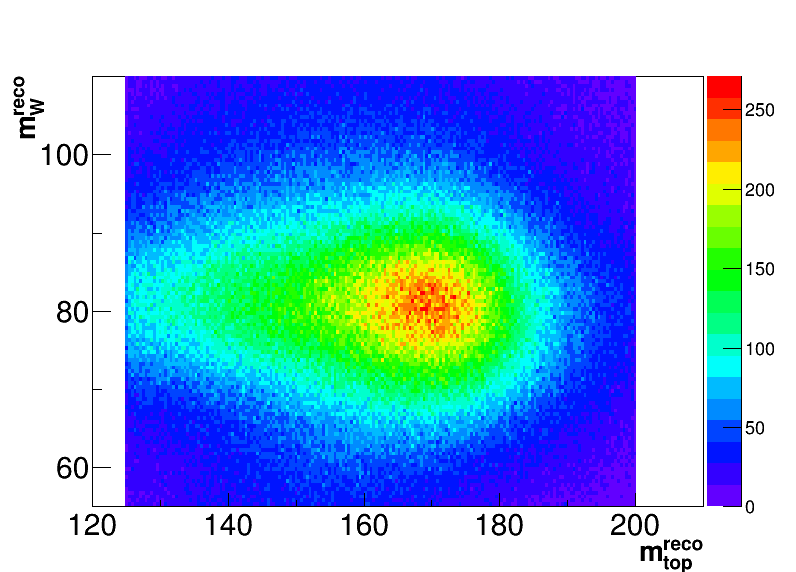
\includegraphics[width=\linewidth]{Pics/PlotCombi/mtopmw.png}
		\caption{Correlation: $m_{top}^{reco}$ and $R_{bq}^{reco}$.} \label{fig:1a}
	\end{subfigure}
	\hspace*{0.1cm}
	\begin{subfigure}{0.35\textwidth}
	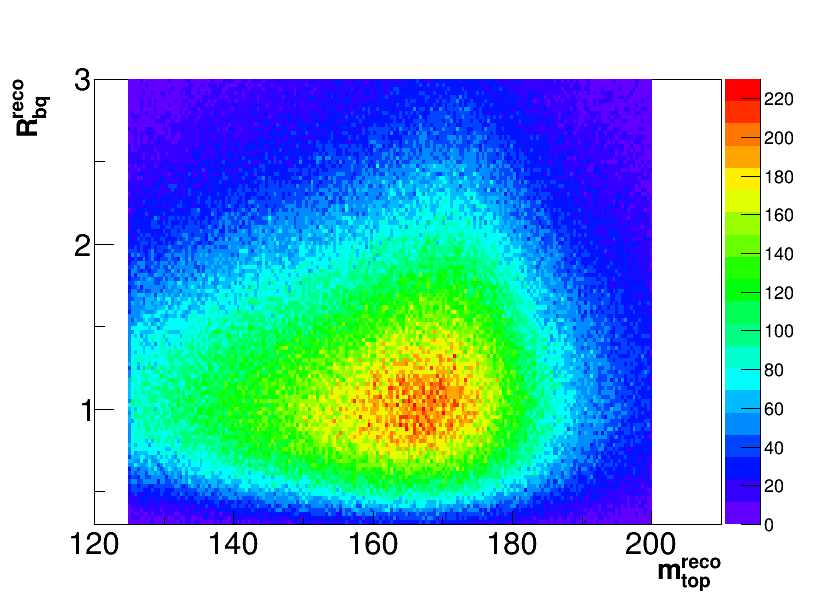
\includegraphics[width=\linewidth]{Pics/PlotCombi/mtopRbq.png}
	\caption{Correlation:  $m_{top}^{reco}$ and $m_{W}^{reco}$.} \label{fig:1b}
	\end{subfigure}

	\begin{subfigure}{0.35\textwidth}
	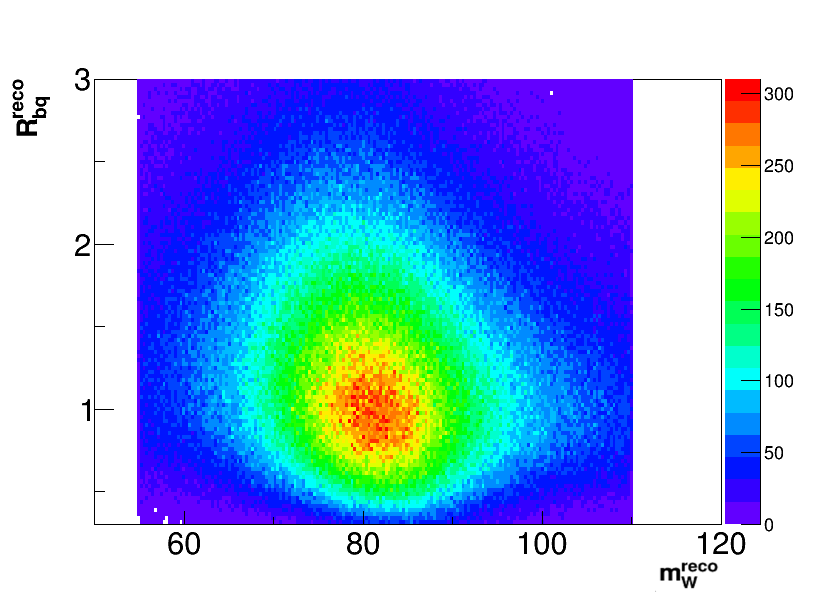
\includegraphics[width=\linewidth]{Pics/PlotCombi/mwRbq2.png}
	\caption{Correlation:  $m_{W}^{reco}$ and $R_{bq}^{reco}$.} \label{fig:1c}
	\end{subfigure}

	\caption{Pair-wise correlation for the observables.}
\end{figure}	
